\subsection{RecConvSiameseNetTraining}\label{subsec:recconvsnet_train}
Having described all previous stages, we delve now into details of the training step for the model we presented in section \vref{subsec:recconvsnet}.
RecConvSiameseNet was trained to minimize categorical cross entropy loss function for $800$ epochs with Adadelta algorithm, learning rate $\eta = 1$, $\rho=0.95$ and $\epsilon=10^{-8}$, and a batch size of $200$. Graph of training/test loss during the epochs is shown in Figure \vref{fig:recconvsnet_loss}, with the final resulting loss being $1.2096$ on the training set and $1.2071$ on the test set.

\begin{figure}
	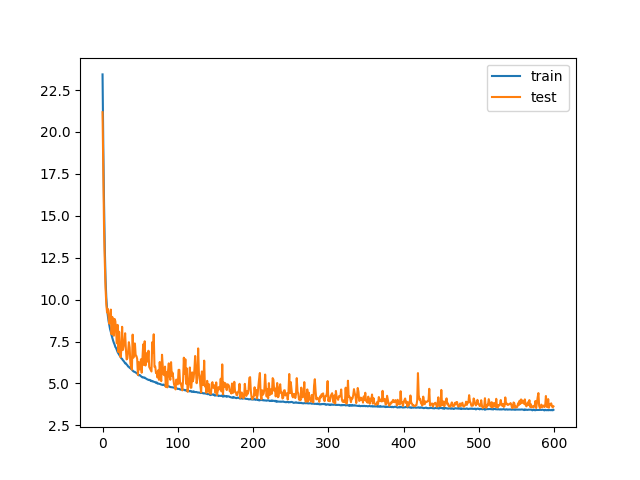
\includegraphics[width=0.5\textwidth]{images/recconvsnet_graph.png}
	\caption{RecConvSiameseNet train/validation loss over the first 600 epochs.}
	\label{fig:recconvsnet_loss}
\end{figure}
As the network architecture is particularly complex and deep, several regularization techniques were applied to reduce overfitting and increase the generalization capabilities of the model:

\begin{itemize}
	\item for the convolutional branch: dropout rate~=~0.5;
	\item for the LSTM branch: dropout rate~=~0.7;
	\item in the first dense layer of the tail: dropout  rate~=~0.5;
	\item $L_1$ loss penalty  on the final activation values with $\lambda = 10^{-5}$;
	\item $L_1$ loss penalty on the weight values of the first dense level of the tail, with $\lambda = 10^{-5}$.
\end{itemize}

\paragraph{Evaluation metrics}
As discussed before, the network is trained using the labels generated by audio forced alignment on the GMM-HMM acoustic models with Viterbi algorithm, so it learns to estimate the posterior probabilities:

$$P(s_t = k \, | \, o_t)$$
for each state $k$, given the frame $o_t$ at each time step $t$. The training labels being artificially generated by GMM-HMM acoustic models, we surely not want the network to (hypothetically) perfectly or almost perfectly match the labels with its predictions, since this would make them completely useless, as they would be no more than an approximation of an already known model predictions (the GMM-HMM model).
It follows from this reasoning that simple accuracy cannot be used as a metric to evaluate the goodness of a neural model underlying a DNN-HMM system, since we are not interested into evaluating the exact match between network-predicted most likely state and the Viterbi-predicted ones.

What we are really interested in quantifying in this context is the model's ability to predict as most likely states those from the acoustic model of a certain speaker, given an audio $o = o_1, o_2, ..., o_T$ belonging to the latter.

The number of states of each speaker GMM-HMM acoustic model being $\statesspeakers = 8$, we used three different metrics to evaluate the performances of RecConvSiameseNet (prior to the SI step), one being widely-used and two custom ones. Each metric is calculated frame-wise, having $0$ as a minimun score and $1$ maximum score on each of them.

\begin{description}
	\item[Top-K accuracy:] the widely-used Top-K accuracy rate with $k = 8$, for each training instance frame $o_t$, it scores $1$ if the real state label $y_t$ is in the top-8 highest probability $P(s_t = q \, | \, o_t)$ values predicted by the network, and $0$ otherwise;
	
	\item[Top-K speaker accuracy:] a slightly modified Top-K accuracy rate with $k = 8$, for each training instance frame $o_t$, it scores $1$ if the real state label $y_t$ or any state label from the same speaker is in the top-8 highest probability $P(s_t = q \, | \, o_t)$ values predicted by the network, and $0$ otherwise;
	
	\item[Number of speaker states in Top-K:] a custom metric that counts, for each training instance frame $o_t$, how much states of the corresponding speaker are in the top-K most likely ones predicted by the network (with $k=8$), divided by the number of states for each speaker $\statesspeakers = 8$ (so we have 0 in case no right state is in the top-8, 0.5 if exactly 4 are, and so on).
\end{description}
Among all the above metrics, \textit{number of speaker states in top-K} is arguably the most meaningful of the three, since it carries the most information, taking into account all the states and giving all frames a different weight between 0 and 1, based on how the network performed on that specific frame. On the other hand, \textit{top-K accuracy} doesn't takes into account every state, and \textit{top-K speaker accuracy} doesn't give different weight if model predicts more than 1 speaker state in the top-K.

Table \vref{tab:reccovsnet_metrics} shows values of each presented metric for the final model, which appear to be quite high. 

\begin{footnotesize}
	\begin{table}
		\centering
		\caption{RecConvSiameseNet's metrics results}
		\begin{tabularx}{0.5\textwidth}{ccc}
			\toprule
			\textbf{Top-8} 				& \textbf{Top-8 speaker} & \textbf{\# States in top-K}    \\
			\midrule
			0.9698	              		& 0.9968                     & 0.9690         \\[0.25cm]
			\bottomrule
		\end{tabularx}
		
	\end{table}\label{tab:reccovsnet_metrics}
\end{footnotesize}